\documentclass{beamer}

\definecolor{theme}{RGB}{6,47,80}
\definecolor{accent}{RGB}{231,83,69}
\definecolor{offblack}{HTML}{262626}
\setbeamercolor{normal text}{fg=offblack}

\usecolortheme[named=theme]{structure}
\usecolortheme{rose}  % inner
\usecolortheme{dolphin}  % outer

% modified version of default frametitle with horizontal separation line
\makeatletter
\setbeamertemplate{frametitle}{
  \ifbeamercolorempty[bg]{frametitle}{}{\nointerlineskip}%
  \@tempdima=\textwidth%
  \advance\@tempdima by\beamer@leftmargin%
  \advance\@tempdima by\beamer@rightmargin%
  \begin{beamercolorbox}[sep=0.3cm,left,wd=\the\@tempdima]{frametitle}
    \usebeamerfont{frametitle}%
    \vbox{}\vskip-2ex%
    \if@tempswa\else\csname beamer@fteleft\endcsname\fi%
    \strut\insertframetitle\strut\par%
    {%
      \ifx\insertframesubtitle\@empty%
      \else%
      {\usebeamerfont{framesubtitle}\usebeamercolor[fg]{framesubtitle}\insertframesubtitle\strut\par}%
      \fi
    }%
    \vskip.45ex%
    \hrule %height .6pt%
    \vskip-1.45ex%
    \if@tempswa\else\vskip-.3cm\fi%
  \end{beamercolorbox}%
}
\makeatother

% clean up footer
\beamertemplatenavigationsymbolsempty
\defbeamertemplate{footline}{custom footline}{
  \usebeamercolor[fg]{page number in head/foot}
  \usebeamerfont{page number in head/foot}
  \quad
  \insertshortauthor\enskip(\insertshortinstitute)
  \hfill
  \insertshorttitle
  \hfill
  \insertframenumber\,/\,\inserttotalframenumber\kern1em\vskip2pt
}
\setbeamertemplate{footline}[custom footline]

\useinnertheme{default}

\setbeamertemplate{itemize items}[circle]
\setbeamercolor{itemize item}{fg=theme!60!white}
\setbeamercolor{itemize subitem}{fg=theme!60!white}

% for backup slides
\usepackage{appendixnumberbeamer}
\renewcommand\appendixname{Backup}

\usepackage{graphicx}
\graphicspath{{../plots/}}

\usepackage{amsmath}
\usepackage{setspace}

\usepackage{tikz}
\usetikzlibrary{calc}
\usetikzlibrary{positioning}
\usetikzlibrary{overlay-beamer-styles}

\usepackage[T1]{fontenc}
% main font
\usepackage[default]{lato}
% improves consistency of Greek letters in math mode
\usepackage{newtxsf}

% alternate font
\usepackage[nosfdefault]{raleway}
% set as the default rm font [even though it really isn't roman]
\renewcommand*\rmdefault{Raleway-TLF}
% and use as the frame title font
\setbeamerfont{frametitle}{family=\rm}

\newcommand{\fullwidth}[1]{
  \begin{columns}
    \column{\paperwidth}
    #1
  \end{columns}
}
\newcommand{\tran}{^\intercal}
\newcommand{\order}[1]{$\mathcal O(10^{#1}$)}
\newcommand{\trento}{T\raisebox{-.5ex}{R}ENTo}
\newcommand{\es}{(\eta/s)}
\newcommand{\zs}{(\zeta/s)}

\title[Bayesian characterization of the initial state and QGP medium]{
  Characterization of the initial state and QGP medium from a combined Bayesian analysis of LHC data at 2.76 and 5.02 TeV
}
\author[J.\ E.\ Bernhard]{Jonah E.\ Bernhard \\ J.\ Scott Moreland, Steffen A.\ Bass}
\institute[Duke U.]{Duke University}
\date{Tuesday 7 February 2017}


\begin{document}


\section{Title}

\begin{frame}[plain,noframenumbering]
  \rm\fontseries{l}
  \centering
  \setstretch{1.4}
  \vspace{.15\textheight}
  {\color{theme}\Large\inserttitle} \\[.05\textheight]
  \insertauthor \\[.1\textheight]
  
\includegraphics[height=.1\textheight]{logos/dukeqcd}
  \hspace{.08\textwidth}
  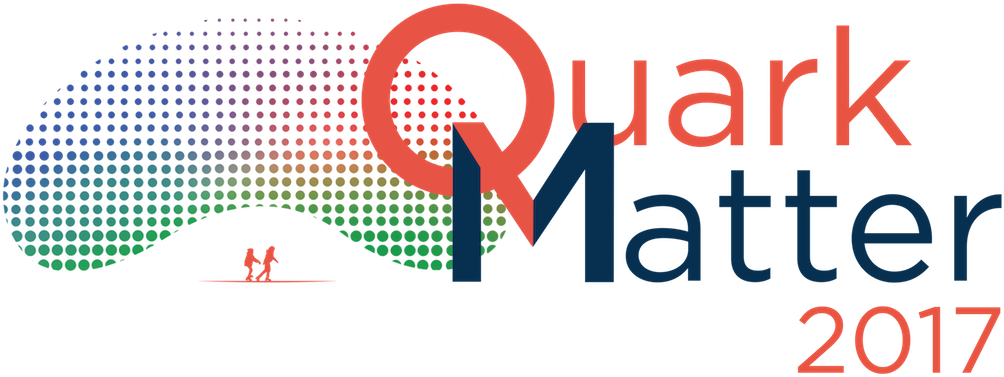
\includegraphics[height=.1\textheight]{logos/qm2017}
\end{frame}


\section{Introduction}

{
\usebackgroundtemplate{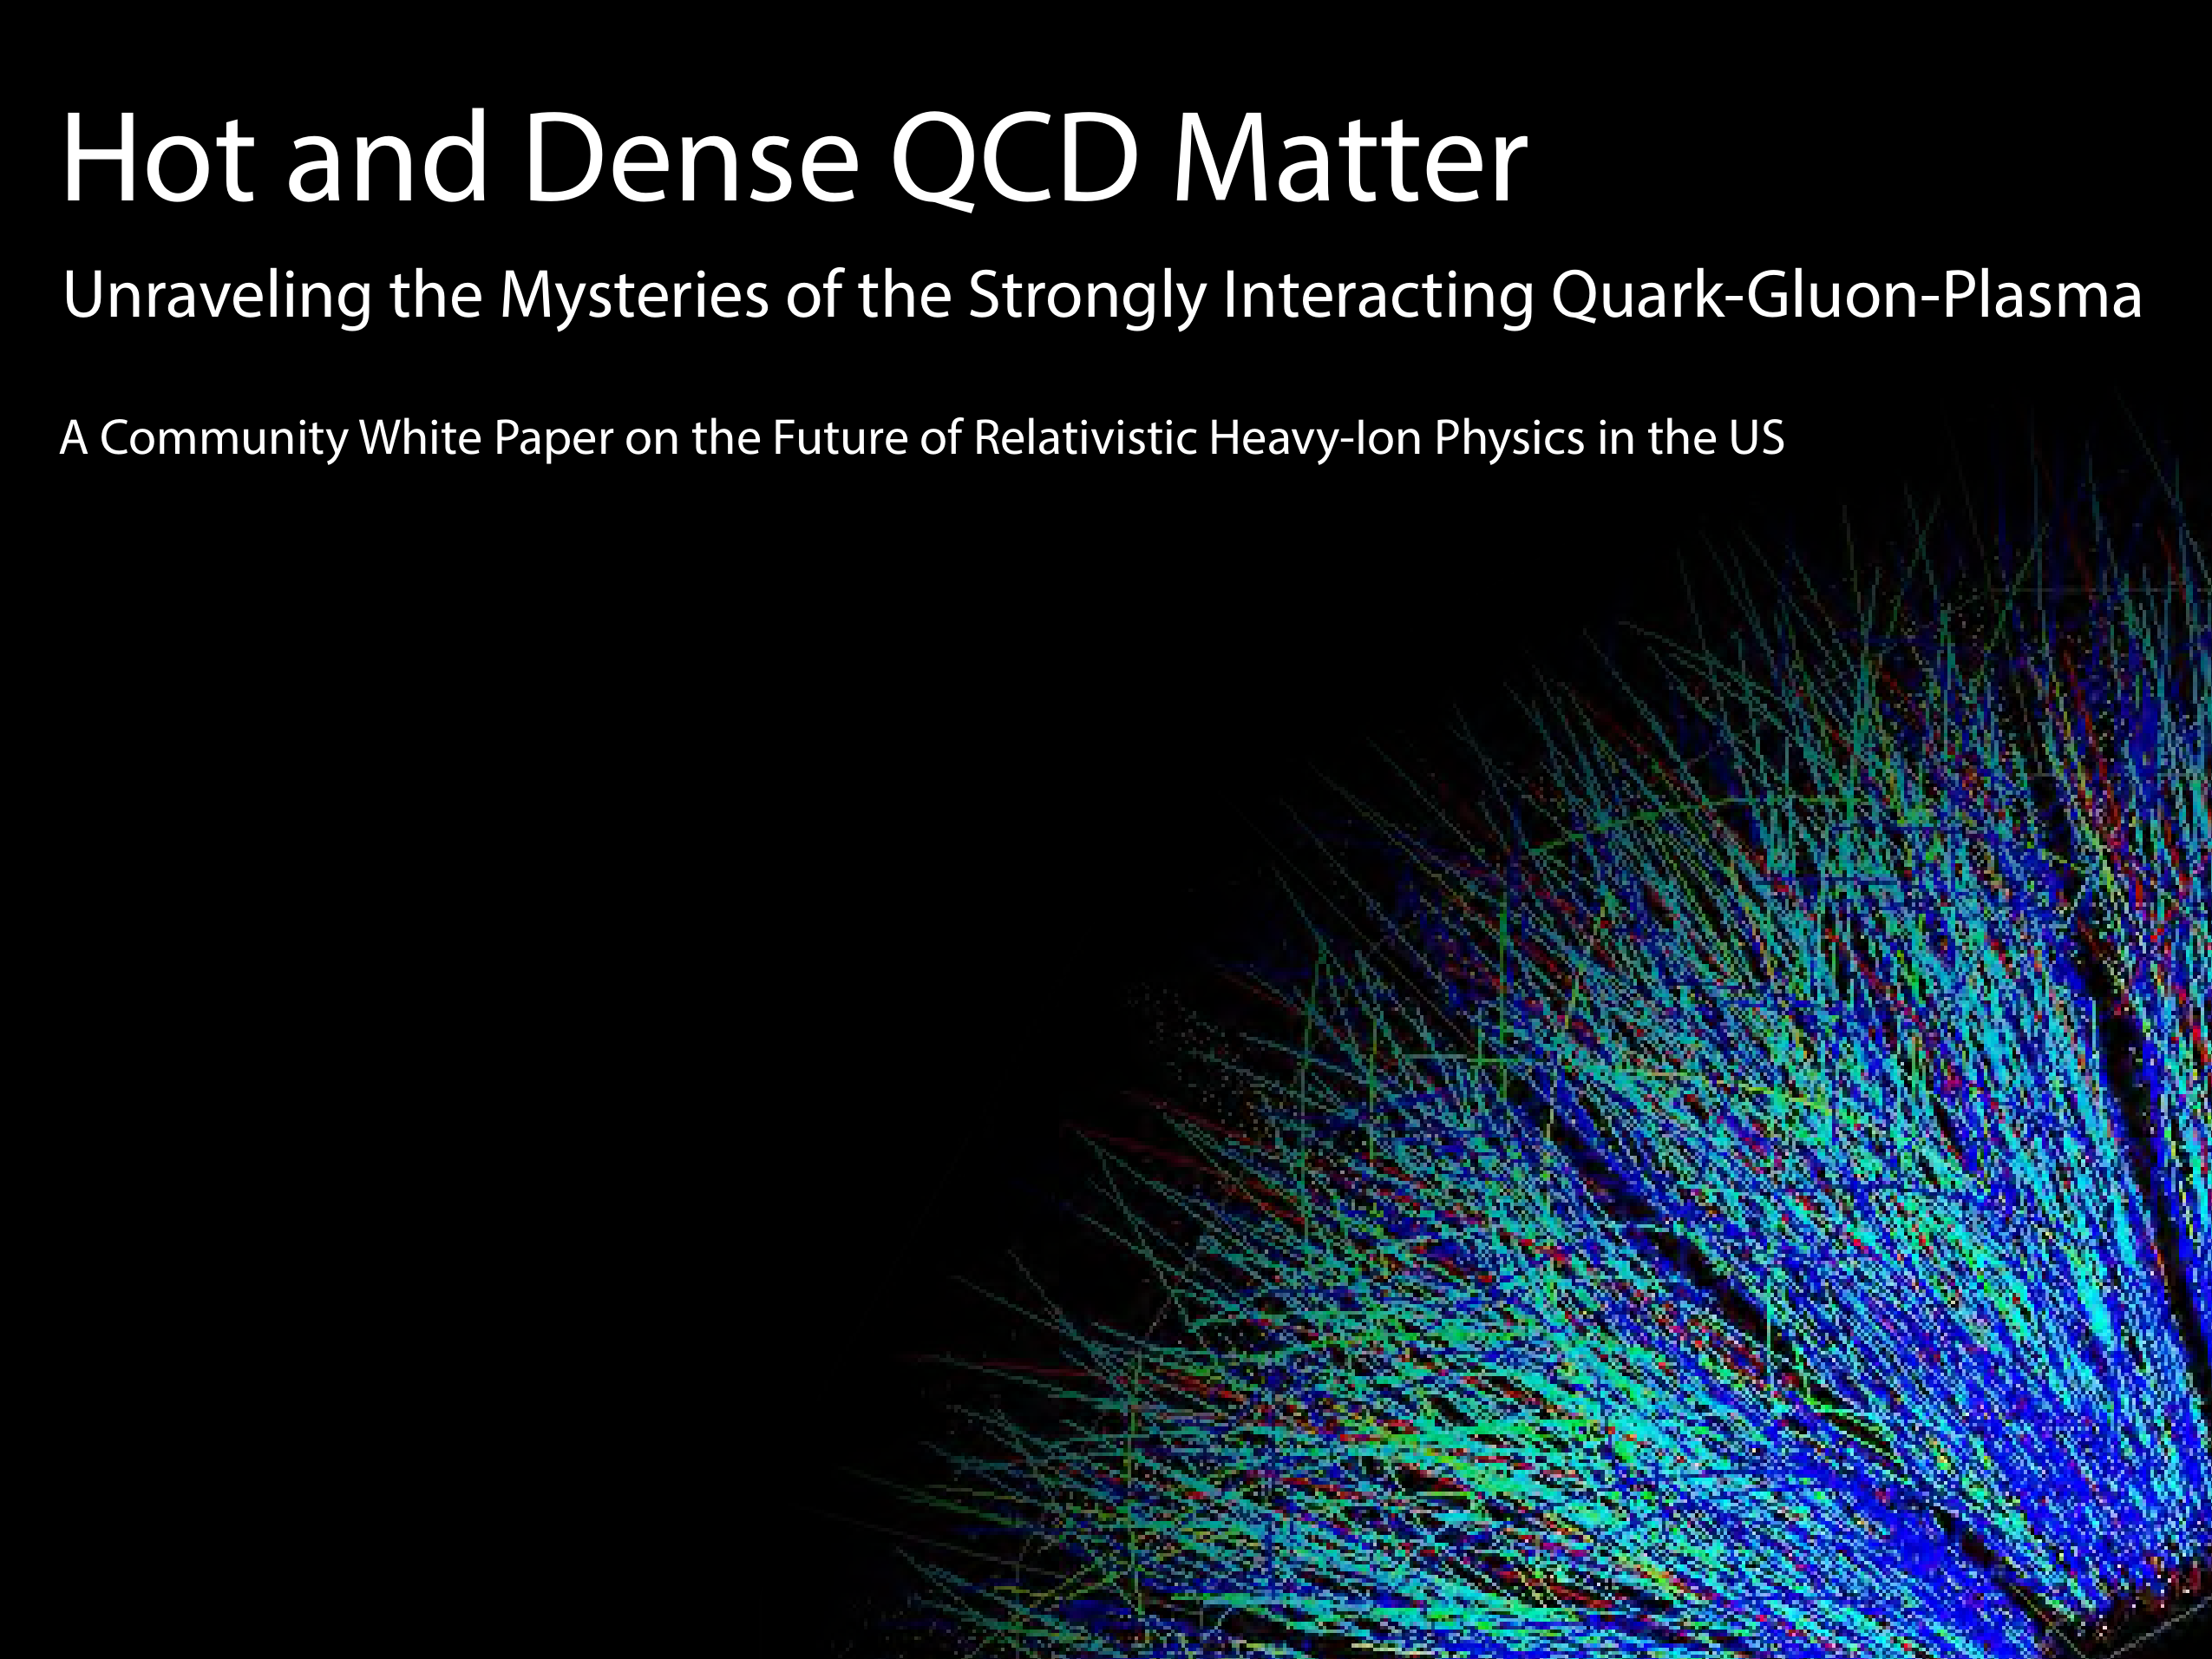
\includegraphics[width=\paperwidth]{whitepaper}}
\begin{frame}[plain]
  \begin{tikzpicture}[remember picture, overlay]
    \node[anchor=west, inner sep=1em, yshift=-2em, text width=.6\paperwidth]
    at (current page.west) {
      \color{white}%
      \small%
      \raisebox{-1ex}{\Huge\color{lightgray}``\ \ }%
      The next 5--10 years of the US relativistic heavy-ion program will deliver\ldots
      the quantitative determination of the transport coefficients of the Quark Gluon
      Plasma, such as the temperature dependent shear-viscosity to entropy-density
      ratio $(\eta/s)(T)$ \ldots
      \raisebox{-2.4ex}{\Huge\color{lightgray}\ \ ''}
    };
  \end{tikzpicture}
\end{frame}
}

\tikzset{
  box/.style={
    align=center,
    inner sep=1ex,
    background default fill=black!10,
    background default text=black!30,
    background fill=theme!15,
    background text=theme,
    fill on=<{1,#1}>,
    text on=<{1,#1}>
  }
}

\newcommand{\boxtitle}[1]{\textbf{#1}\\[.5ex]}

\begin{frame}<1>[label=flowchart]{Overview}
  \vspace{1em}
  \makebox[\textwidth]{
  \begin{tikzpicture}
    \node[box=3] (input) at (4.5, 6) {
      \boxtitle{Input parameters}
      QGP properties
    };
    \node[box=2] (model) at (8, 4) {
      \boxtitle{Model}
      heavy-ion collision \\
      spacetime evolution
    };
    \node[box=4] (gp) at (1.5, 4) {
      \boxtitle{Gaussian process emulator}
      surrogate model
    };
    \node[box=4] (mcmc) at (3.5, 2) {
      \boxtitle{MCMC}
      calibrate model to data
    };
    \node[box=5] (posterior) at (8, .5) {
      \boxtitle{Posterior distribution}
      quantitative estimates \\
      of each parameter
    };
    \node[box=3] (exp) at (.5, .3) {
      \boxtitle{Experimental data}
      LHC Pb-Pb collisions
    };
    \begin{scope}[color=black!70, ->, semithick]
      \draw (input) -| (model);
      \draw (model) -- (gp);
      \draw (input) -| (gp);
      \draw
        let \p1 = (gp.south), \p2 = (mcmc.north), \p3 = ($(\p1)!.5!(\p2)$) in
        (\p1) -- (\x1, \y3)  -| (\p2);
      \draw (exp) |- (mcmc);
      \draw (mcmc) -| (posterior);
    \end{scope}
  \end{tikzpicture}
  }
\end{frame}


\section{Method}

\againframe<2>[noframenumbering]{flowchart}

\tikzset{fade/.style={opacity=.25}}
\newcommand{\eventframes}[1]{
  \foreach \style [count=\n from 0] in #1 {
    \tikz\node[\style] {\includegraphics[height=5em]{eventframes/\n}};
    \hfill
  } \\
}

\begin{frame}[t]{Model}
  \eventframes{{,,,,,,}}
  \medskip
  \begin{enumerate}
    \item Initial conditions \hfill $t = 0^+$ \\
      \begin{itemize}
        \item Entropy deposition
      \end{itemize}
    \item Pre-equilibrium \hfill $t < 1$ fm/$c$
      \begin{itemize}
        \item Early-time dynamics and thermalization
      \end{itemize}
    \item Hydrodynamics \hfill $1 < t < 10$ fm/$c$
      \begin{itemize}
        \item Hot and dense QGP
      \end{itemize}
    \item Particlization and hadronic phase \hfill $10 < t < 100$ fm/$c$
      \begin{itemize}
        \item Conversion to particles
        \item Expanding and cooling gas
      \end{itemize}
  \end{enumerate}
\end{frame}

\begin{frame}{\trento: parametric initial condition model}
  \begin{columns}
    \column{.65\textwidth}
    \textbf{Ansatz}: entropy density proportional to \textbf{generalized mean} of local nuclear density
    \begin{equation*}
      s \propto \biggl( \frac{T_A^p + T_B^p}{2} \biggr)^{1/p}
    \end{equation*}
    $p \in (-\infty, \infty)$ = tunable parameter; \\
    varying $p$ mimics other models:
    \begin{itemize}
      \item $p = 1 \,\implies\, s \propto T_A + T_B$ \\
        wounded nucleon model
      \item $p = 0 \,\implies\, s \propto \sqrt{T_A T_B}$ \\
        similar to IP-Glasma, EKRT
      \item Previous work: $p = 0.0 \pm 0.2$ \\[1ex]
        \tiny
        PRC 92 011901 [1412.4708] \quad
        PRC 94 024907 [1605.03954]
    \end{itemize}
    \medskip
    \footnotesize
    See talk by S.~Moreland, Wed.~10:40
    \column{.28\textwidth}
    \vspace{1em}
    \includegraphics[width=\textwidth]{trento_events}
  \end{columns}
\end{frame}

\begin{frame}[t]{Pre-equilibrium}
  \eventframes{{fade,,,fade,fade,fade,fade}}
  \begin{center}
    \bf Free-streaming approximation
  \end{center}
  \begin{itemize}
    \setlength{\itemsep}{1ex}
    \item Expanding, noninteracting gas of massless partons
    \item Sudden thermalization and switch to hydrodynamics at tunable time $\tau_\text{fs}$
    \item Smooths out initial density, increases radial flow velocity
  \end{itemize}
  \tiny\flushright PRC 80 034902 [0812.3393] \quad PRC 92 064906 [1504.02160]
\end{frame}

\begin{frame}[t]{Hydrodynamics}
  \eventframes{{fade,fade,,,,fade,fade}}
  \vspace{-1ex}
  \begin{center}
    {\bf OSU VISH2+1} \\[1ex]
    \tiny
    PRC 77 064901 [0712.3715] \quad
    CPC 199 61 [1409.8164]
  \end{center}
  \vspace{-1ex}
  \begin{itemize}
    \setlength{\itemsep}{1ex}
    \item Boost-invariant viscous hydrodynamics
    \item Temperature-dependent shear and bulk viscosities
    \item Hybrid equation of state
      \begin{itemize}
        \item HRG EOS at low temperature
        \item HOTQCD lattice EOS at high temperature \\
          {\tiny PRD 90 094503 [1407.6387]}
      \end{itemize}
  \end{itemize}
\end{frame}

\begin{frame}{Temperature-dependent viscosities}
  \vspace{-1em}
  \begin{columns}[t]
    \column{.5\textwidth}
    \begin{center}
      \bf Shear
    \end{center}
    Tunable minimum at $T_c$, slope, and curvature
    \begin{align*}
      &\es(T) = \es_\text{min} + {} \\
      &\quad \es_\text{slope}(T - T_c)
        \times \biggl( \frac{T}{T_c} \biggr)^{\es_\text{crv}}
    \end{align*}
    \includegraphics[width=\textwidth]{region_shear_examples}
    \column{.5\textwidth}
    \begin{center}
      \bf Bulk
    \end{center}
    Cauchy distribution with peak at $T_c$, tunable height and width
    \begin{equation*}
      \zs(T) = \frac{
        \zs_\text{max}
      }{
        1 + \biggl( \dfrac{T - T_c}{\zs_\text{width}} \biggr)^2
      }
    \end{equation*}
    \includegraphics[width=\textwidth]{region_bulk_examples}
  \end{columns}
\end{frame}

\begin{frame}[t]{Particlization and hadronic phase}
  \eventframes{{fade,fade,fade,fade,fade,,}}
  \medskip
  Convert hydrodynamic medium $\rightarrow$ particles at tunable $T_\text{switch}$
  \begin{itemize}
    \item Particle species and momenta sampled from thermal hadron resonance gas (Cooper-Frye)
    \item Novel implementation of shear and bulk viscous corrections based on relaxation-time approximation \\
      {\tiny PRC 82 044901 [1003.0413] \quad PRC 85 044909 [1109.5181] \quad PRC 83 044910 [1012.5927]}
    \item Masses of unstable resonances sampled from Breit-Wigner distribution
  \end{itemize}
  \bigskip
  Hadronic scatterings and decays: UrQMD
\end{frame}

\againframe<3>[noframenumbering]{flowchart}

\begin{frame}{Input parameters}
  \definecolor{emph}{rgb}{.91,.41,.17}
  \begin{columns}
    \column{.55\textwidth}
    Initial condition
    \begin{itemize}
      \item \trento\ entropy deposition $p$
      \item Multiplicity fluctuation $\sigma_\text{fluct}$
      \item Gaussian nucleon width $w$
    \end{itemize}
    \medskip
    Pre-equilibrium
    \begin{itemize}
      \item Free streaming time $\tau_\text{fs}$
    \end{itemize}
    \medskip
    QGP medium
    \begin{itemize}
      \item $\eta/s$ min, slope, curvature
      \item $\zeta/s$ max, width
      \item $T_\text{switch}$ (hydro to UrQMD)
    \end{itemize}
    \column{.5\textwidth}
    \begin{center}
      \textbf{Latin hypercube design}
    \end{center}
    500 semi-random, space-filling parameter points;
    ${\sim}3 \times 10^4$ min-bias events per point \\[1em]
    \includegraphics{design}
  \end{columns}
\end{frame}

\begin{frame}{Observables}
  \begin{center}
    All experimental data from the ALICE collaboration at the LHC \\
    Pb-Pb collisions at $\sqrt s = 2.76$ and 5.02 TeV
  \end{center}
  \begin{columns}
    \column{.6\textwidth}
    Centrality dependence of: \\[1ex]
    \begin{itemize}
      \setlength{\itemsep}{1.5ex}
      \item Charged particle yields $dN_\text{ch}/d\eta$ \\
        {\tiny PRL 106 032301 [1012.1657], PRL 116 222302 [1512.06104]}
      \item Identified particle ($\pi$, $K$, $p$) yields $dN/dy$
        and mean transverse momenta $\langle p_T \rangle$ (2.76 TeV only) \\
        {\tiny PRC 88 044910 [1303.0737]}
      \item Anisotropic flow cumulants $v_n\{2\}$ \\
        {\tiny PRL 116 132302 [1602.01119]}
    \end{itemize}
    \column{.4\textwidth}
    \centering
    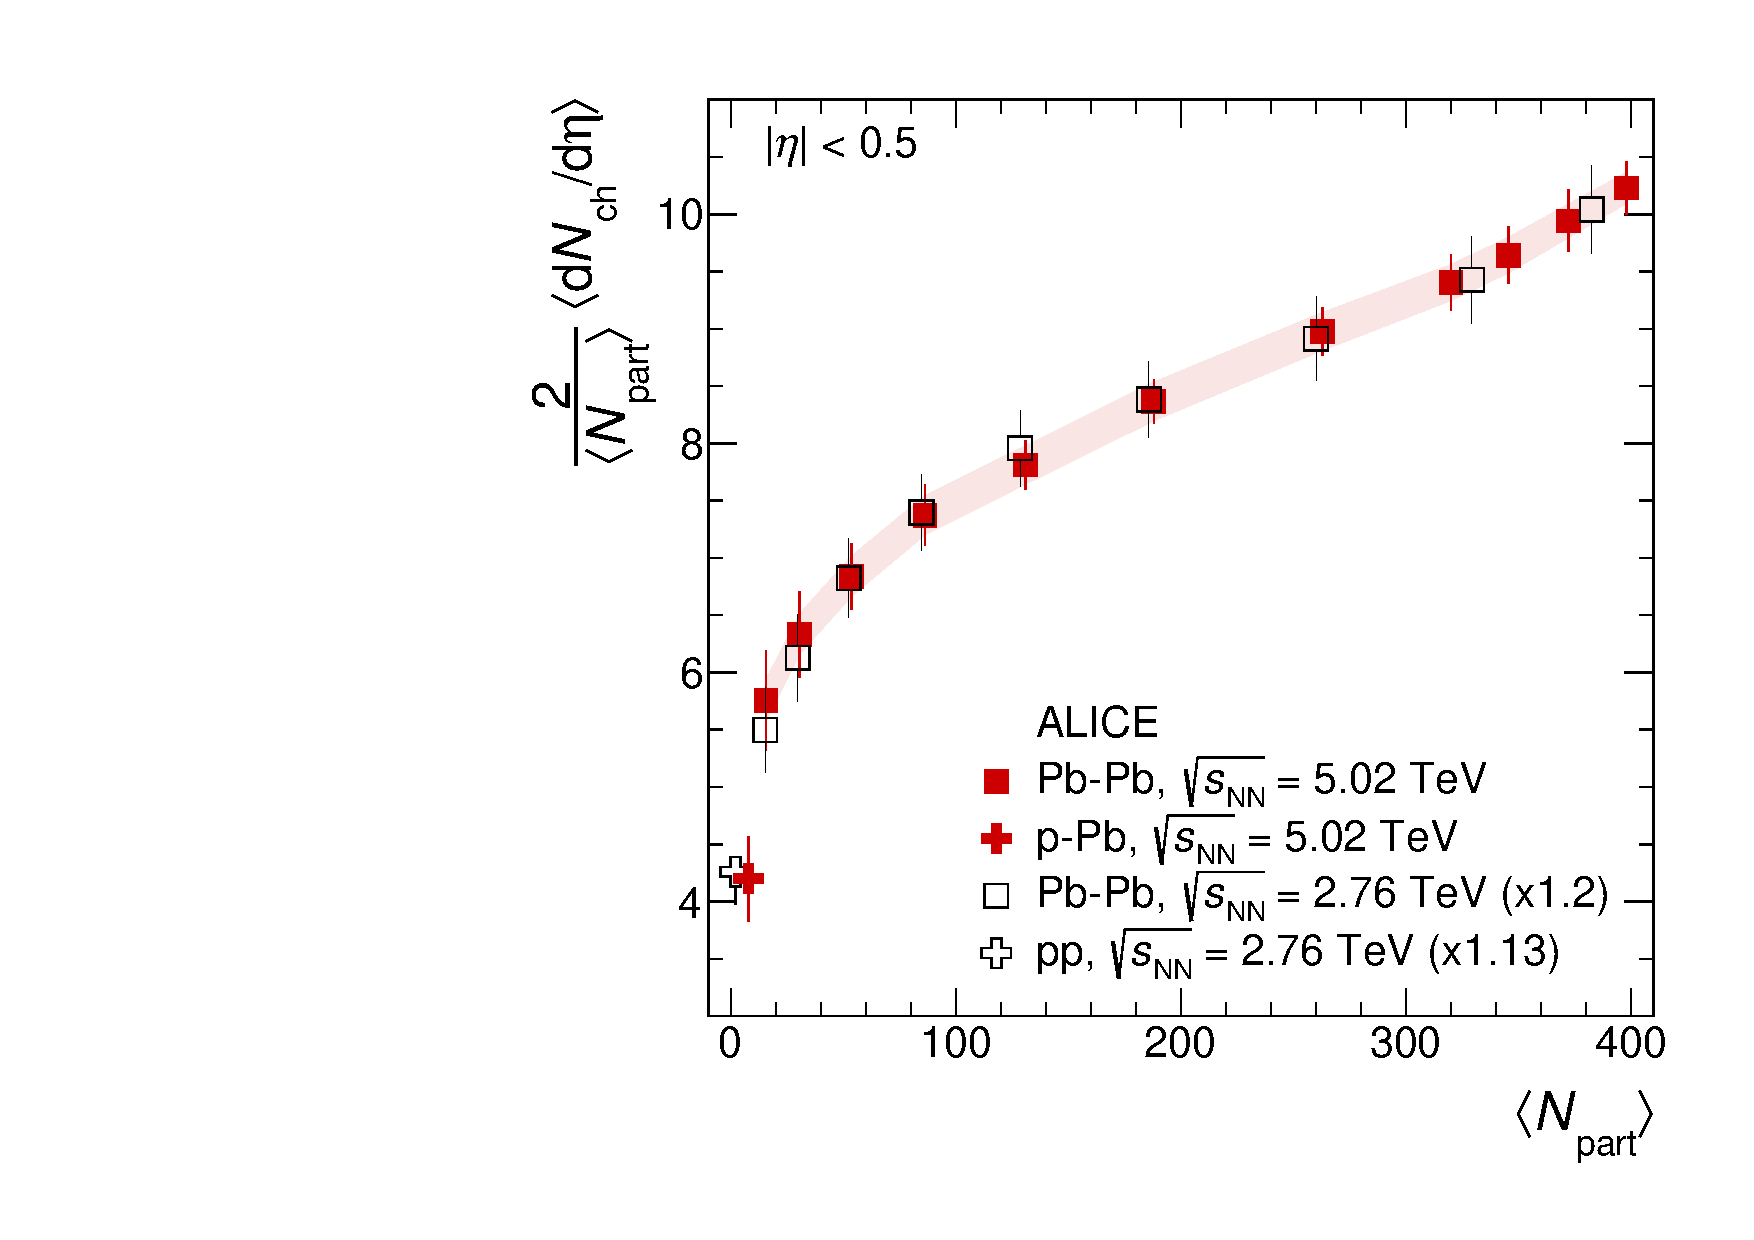
\includegraphics[height=.25\textheight]{exptfigs/nch}
    \hfill
    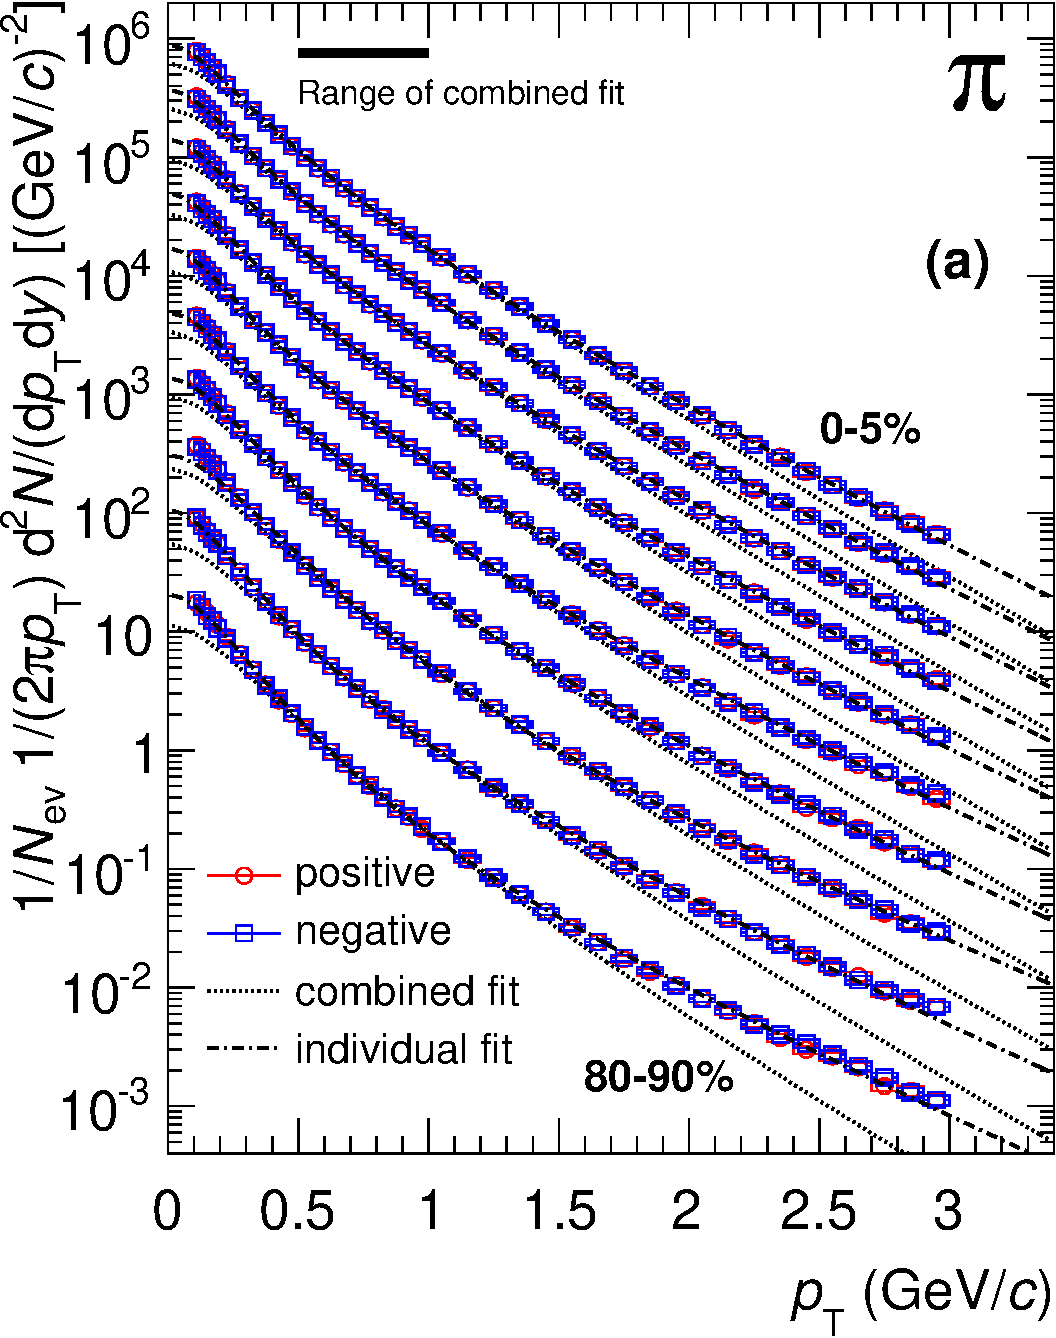
\includegraphics[height=.25\textheight]{exptfigs/spectra} \\
    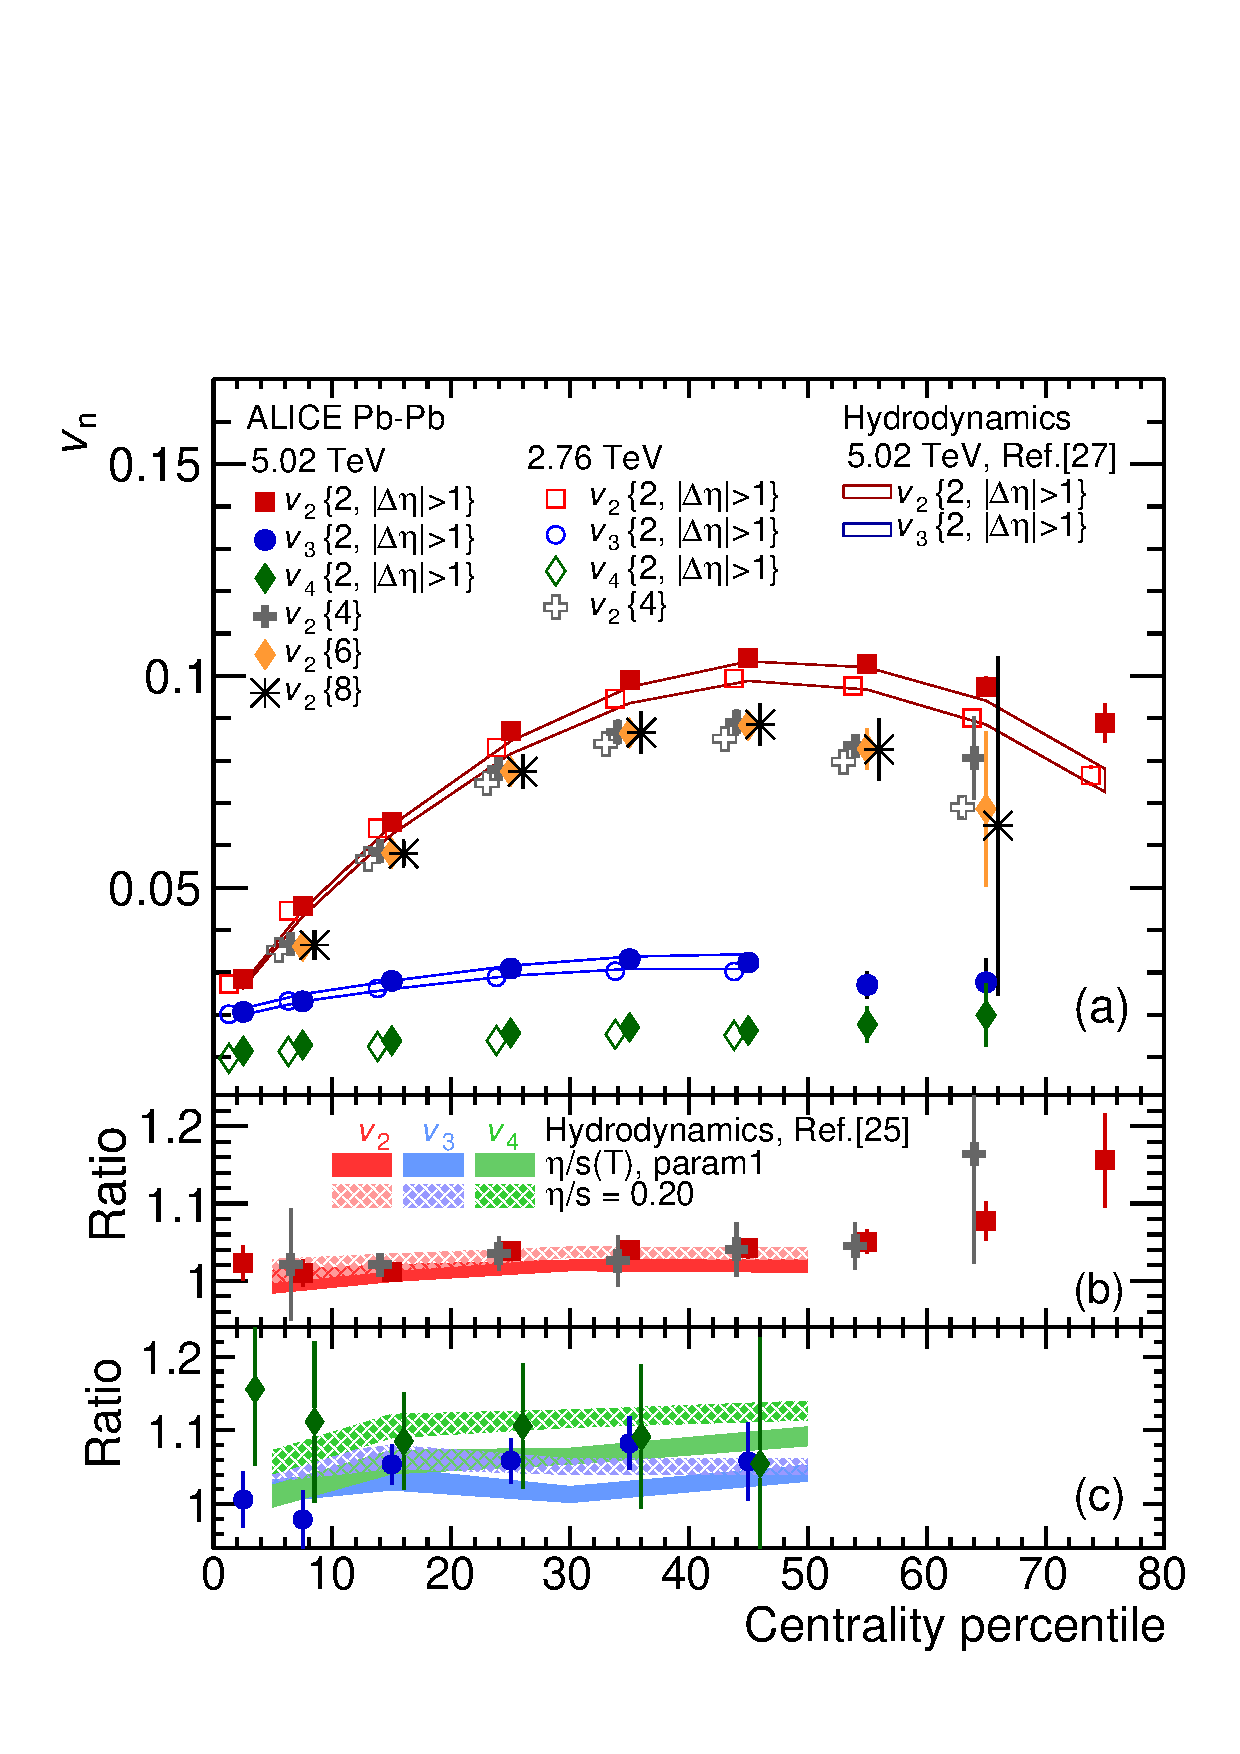
\includegraphics[height=.4\textheight]{exptfigs/flow}
  \end{columns}
\end{frame}

\begin{frame}<1>[label=observables]{
    \only<1-2>{Training data}
    \only<3>{Posterior samples}
}
  \vspace{1em}
  \fullwidth{
    \centering
    \only<1-2>{Model calculations at each design point}
    \only<3>{Emulator predictions from calibrated posterior}
    \\[1em]
    \includegraphics<1-2>{observables_design}
    \includegraphics<3>{observables_posterior}
  }
\end{frame}

\againframe<4>[noframenumbering]{flowchart}

\begin{frame}{Gaussian process emulator}
  \vspace{1em}
  \begin{columns}[c]
    \column{.58\textwidth}
    Gaussian process:
    \begin{itemize}
      \item Stochastic function: maps inputs to normally-distributed outputs
      \item Specified by mean and covariance functions
    \end{itemize}
    \bigskip
    As a model emulator:
    \begin{itemize}
      \item Non-parametric interpolation
      \item Predicts \emph{probability distributions}
        \begin{itemize}
          \item Narrow near training points, \\ wide in gaps
        \end{itemize}
      \item Fast surrogate to actual model
    \end{itemize}
    \column{.45\textwidth}
    \includegraphics{gp}
  \end{columns}
\end{frame}

\newcommand{\ydiff}{(\mathbf y - \mathbf y_\text{exp})}

\begin{frame}{Bayesian model calibration}
  \begin{center}
    \textbf{Bayes' theorem} \\
    posterior ${}\propto{}$ likelihood ${}\times{}$ prior
  \end{center}
  Prior = flat in design space \\[1ex]
  Likelihood${} \propto \exp\bigl[ -\frac{1}{2} \ydiff\tran \Sigma^{-1} \ydiff \bigr]$ \\[.5ex]
  \begin{itemize}
    \item $\Sigma = \text{covariance matrix} = \Sigma_\text{experiment} + \Sigma_\text{model}$
    \item $\Sigma_\text{experiment} = {}$stat (diagonal) + sys (non-diagonal)
    \item $\Sigma_\text{model}$ conservatively estimated as 5\% (to be improved)
  \end{itemize}
  \begin{center}
    \textbf{Markov chain Monte Carlo} \\[1ex]
    Construct posterior distribution by MCMC sampling \\
    (weighted random walk through parameter space)
  \end{center}
\end{frame}

\section{Results}

\againframe<2-3>{observables}

\againframe<5>[noframenumbering]{flowchart}

\begin{frame}<1>[label=posterior, plain]
  \centering
  \includegraphics[height=\paperheight]<1-2>{posterior}
  \includegraphics[height=\paperheight]<3>{posterior_withnorm}
  \begin{tikzpicture}[remember picture, overlay]
    \node[below left=1em and 2.2em of current page.north east, color=theme, font=\Large\rm]
    (title) {
      Posterior distribution
    };
    \node[below=1ex of title, anchor=north, font=\small, align=left] {
      \only<1>{%
        Diagonals: prob.\ dists.\ of each param. \\
        Off-diagonals: correlations b/w pairs \\[1ex]
        Estimated values: medians \\
        Uncertainties: 90\% credible intervals
      }
      \only<2>{Much more information here!}
      \only<3>{with normalization factors}
    };
  \end{tikzpicture}
\end{frame}

\begin{frame}{Initial entropy deposition}
  \begin{columns}
    \column{.65\textwidth}
    \includegraphics{posterior_p}
    \column{.3\textwidth}
    \begin{equation*}
      s \propto \Biggl( \frac{T_A^p + T_B^p}{2} \Biggr)^{1/p}
    \end{equation*}
  \end{columns}
  \medskip
  \begin{itemize}
    \setlength{\itemsep}{1ex}
    \item Entropy deposition $\sim$ geometric mean of local nuclear density $\sqrt{T_A T_B}$
    \item Uncertainty halved from previous work
    \item Corroborates eccentricity scaling of IP-Glasma and EKRT
  \end{itemize}
\end{frame}

\begin{frame}{Shear viscosity}
  \begin{equation*}
    \es(T) = \es_\text{min} + \es_\text{slope}(T - T_c) \times \biggl( \frac{T}{T_c} \biggr)^{\es_\text{crv}}
  \end{equation*}
  \begin{columns}
    \column{.4\textwidth}
    \includegraphics[width=\textwidth]{posterior_shear}
    \column{.6\textwidth}
    \includegraphics[width=\textwidth]{region_shear}
  \end{columns}
  \small
  \begin{itemize}
    \item Zero $\eta/s$ excluded; min consistent with AdS/CFT
    \item Constant $\eta/s$ excluded
    \item Best constrained $T \lesssim 0.23$ GeV
    \item RHIC data could disambiguate slope and curvature
  \end{itemize}
\end{frame}

\begin{frame}{Bulk viscosity}
  \begin{equation*}
    \zs(T) = \frac{
      \zs_\text{max}
    }{
      1 + \biggl( \dfrac{T - T_c}{\zs_\text{width}} \biggr)^2
    }
  \end{equation*}
  \begin{columns}
    \column{.4\textwidth}
    \includegraphics[width=\textwidth]{posterior_bulk}
    \column{.6\textwidth}
    \includegraphics[width=\textwidth]{region_bulk}
  \end{columns}
  \begin{itemize}
    \item Can be ``tall'' or ``wide'', but not both
    \item Short and wide (green) slightly favored
  \end{itemize}
  \scriptsize\flushright See also talk by G.~Denicol, Wed.~17:30
\end{frame}

\againframe<2>[plain,noframenumbering]{posterior}

\begin{frame}[plain,t]
  \fullwidth{
    \centering
    \includegraphics{observables_map}
  }
  \bigskip
  \scriptsize
  \setbeamercolor{lightbg}{bg=theme!10!white}
  \begin{beamercolorbox}[sep=1ex]{lightbg}
    \trento\ $p = 0$
    \hfill
    $\sigma_\text{fluct} = 1$
    \hfill
    $w = 0.9$ fm
    \hfill
    $\tau_\text{fs} = 0.6$ fm/$c$
    \hfill
    $T_\text{switch} = 150$ MeV
    \\[1ex]
    $\eta/s$ min = 0.06, \enskip slope = 2.2 GeV$^{-1}$, \enskip crv = $-0.4$
    \hfill
  $\zeta/s$ max = 0.015, \enskip width = 0.01 GeV
  \end{beamercolorbox}
\end{frame}

\begin{frame}{Flow correlations}
  Correlation between event-by-event fluctuations of the magnitudes of flow harmonics $m$ and $n$:
  \begin{equation*}
    \text{SC}(m, n) = \langle v_m^2 v_n^2 \rangle  - \langle v_m^2 \rangle \langle v_n^2 \rangle
  \end{equation*}
  \includegraphics{flow_corr} \\
  \tiny\flushright Data: ALICE, PRL 117 182301 [1604.07663]
\end{frame}


\begin{frame}{More flow observables}
  \includegraphics{flow_extra}
  \tiny\flushright Data: ALICE, PRL 107 032301 [1105.3865]; PRL 116 132302 [1602.01119]
\end{frame}


\section{Conclusion}

\begin{frame}{Summary and outlook}
  \vspace{1em}
  \begin{itemize}
    \item Global, multi-parameter fit of event-by-event collision model to diverse experimental data at 2.76 and 5.02 TeV
    \item Constrained initial state entropy deposition, fluctuations, and granularity
    \item Estimated temperature dependence of QGP shear and bulk viscosities
      \begin{itemize}
        \item Excluded both zero and constant $\eta/s$
        \item Found preference for short, wide $\zeta/s$ peak
      \end{itemize}
  \end{itemize}
  \begin{itemize}
    \item Include RHIC data to further constrain transport coefficients
    \item Improve uncertainty quantification
  \end{itemize}
  \begin{center}
    This project is open source! \\
    \url{https://github.com/jbernhard/qm2017}
  \end{center}
\end{frame}


\appendix

\againframe<3>[plain]{posterior}

\begin{frame}{Uncertainty quantification}
  Given a set of experimental uncertainties $\{\sigma_i\}$, what is the covariance matrix $\Sigma$? \\[.5ex]
  In general:
  \begin{equation*}
    \Sigma_{ij} = c_{ij} \sigma_i \sigma_j
  \end{equation*}
  where $c_{ij}$ = correlation coefficient between observations $i,j$
  \begin{itemize}
    \item Statistical (uncorrelated) uncertainty
      \begin{equation*}
        c_{ij} = \delta_{ij} \quad\implies\quad \Sigma_\text{stat} = \text{diag}(\sigma_i^2)
      \end{equation*}
    \item Systematic uncertainty: assume Gaussian correlation function
      \begin{equation*}
        c_{ij} = \exp\Biggl[ -\frac{1}{2} \biggl( \frac{x_i - x_j}{100} \biggr)^2 \Biggr]
      \end{equation*}
      where $x_i$ is the centrality \% midpoint of observation $i$
  \end{itemize}
\end{frame}

\begin{frame}{Conditioning a Gaussian process}
  \newcommand{\y}{\mathbf y}
  Given
  \begin{itemize}
    \item training input points $X$
    \item observed training outputs $\y$ at $X$
    \item covariance function $\sigma$
  \end{itemize}
  the predictive distribution at arbitrary test points $X_*$ is the multivariate-normal distribution
  \begin{align*}
    \y_* &\sim \mathcal N(\boldsymbol\mu, \Sigma) \\
    \boldsymbol\mu &= \sigma(X_*, X)\sigma(X, X)^{-1}\y \\
    \Sigma &= \sigma(X_*,X_*) - \sigma(X_*,X)\sigma(X,X)^{-1}\sigma(X,X_*)
  \end{align*}
\end{frame}

\begin{frame}{Multivariate output}
  \begin{columns}
    \column{.55\textwidth}
    Many highly correlated outputs \\
    $\rightarrow$ \textbf{principal component analysis} \\[1em]
    PCs = eigenvectors of sample covariance matrix
    \begin{equation*}
      Y\tran Y = U \Lambda U\tran
    \end{equation*}
    Transform data into orthogonal, uncorrelated linear combinations
    \begin{equation*}
      Z = \sqrt m \, YU
    \end{equation*}
    Emulate each PC independently
    \column{.45\textwidth}
    Example transformation of two observables \\[2ex]
    \includegraphics{pca}
  \end{columns}
\end{frame}


\end{document}
